\lstdefinelanguage{plaintext}{
  sensitive=false,
  comment=[l]{//},
  morecomment=[s]{/*}{*/},
  identifierstyle=\color{black},
  morestring=[b]',
  morestring=[b]"
}

\lstset
{ 
    language=plaintext,
    basicstyle=\footnotesize,
    numbers=left,
    stepnumber=1,
    showstringspaces=false,
    tabsize=1,
    breaklines=true,
    breakatwhitespace=false,
    frame=leftline
}

\chapter{Analisis}
\label{chap:analisis}
%blm fix
Pada bab ini dijelaskan mengenai analisis aplikasi sejenis, analisis penggunaan Git Command Line, analisis penggunaan JGit, analisis penggunaan Selenium WebDriver, analisis Command Line Options, dan prapengujian. 

\section{Analisis Aplikasi Sejenis}
\label{sec:analisis_aplikasi_sejenis}
Saat skripsi ini dibuat, aplikasi sejenis yang digunakan untuk membangkitkan animasi adalah Gource.  
Proyek perangkat lunak ditampilkan oleh Gource sebagai animasi pohon, dimana pusatnya adalah \textit{root directory} dari proyek perangkat lunak\cite{Gource}. Direktori ditampilkan sebagai \textit{branch}, sedangkan \textit{file} ditampilkan sebagai \textit{leaf}. Developer dapat terlihat di \textit{working tree} pada saat mereka berkontribusi untuk proyek.

\begin{figure}[H]
	\centering
		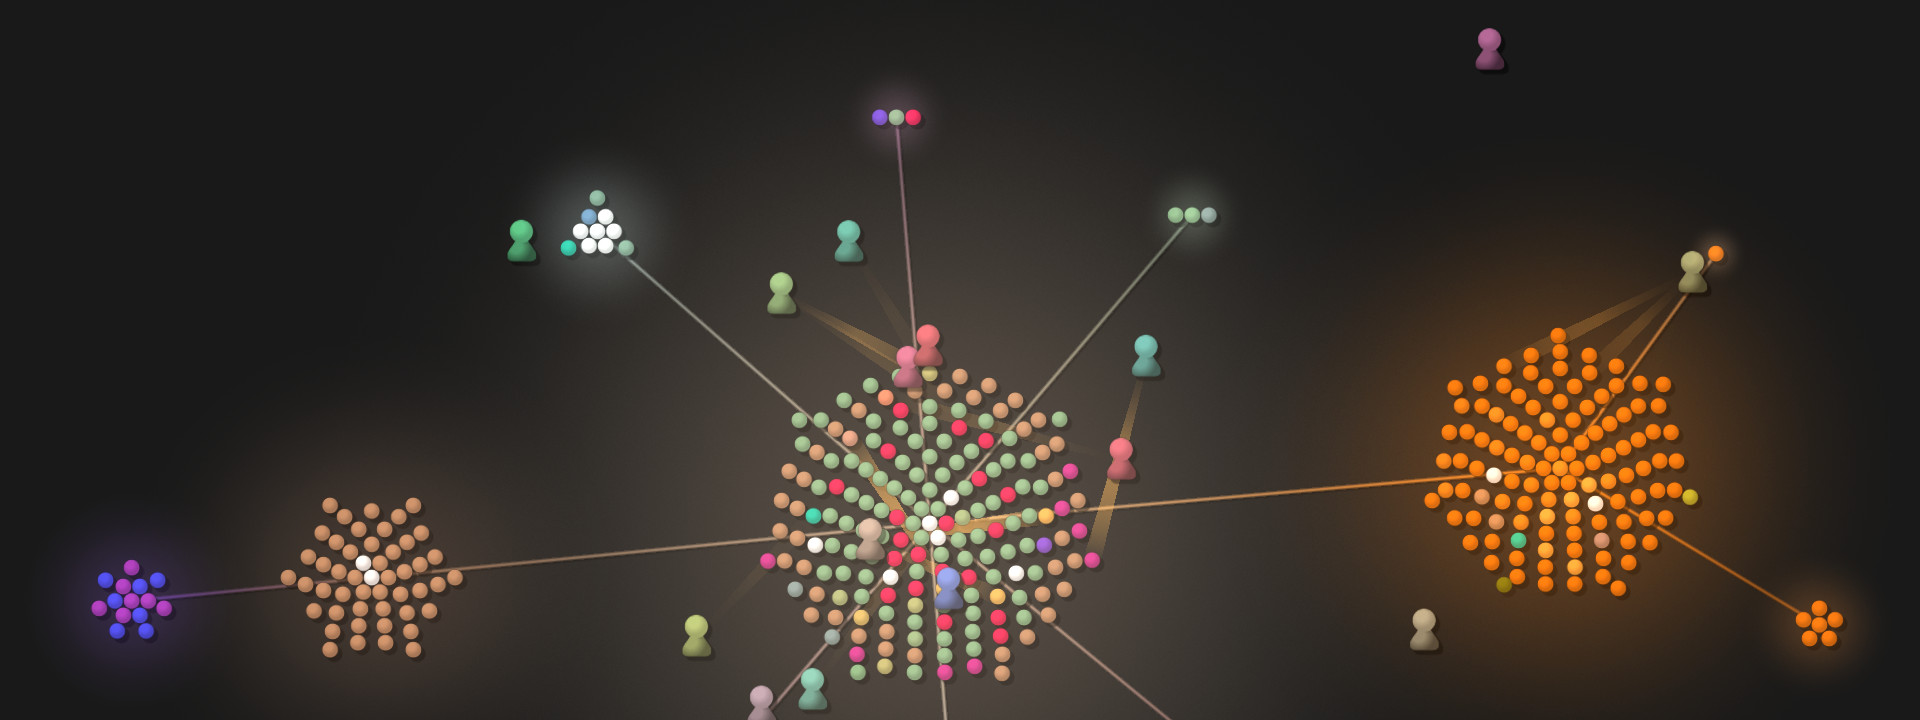
\includegraphics[scale=0.2]{Gambar/gource.jpg}
	\caption{Visualisasi proyek perangkat lunak menggunakan Gource.}
	\label{fig:gource}
\end{figure}

Gambar \ref{fig:gource} menunjukkan contoh visualisasi proyek perangkat lunak menggunakan Gource. Efek cahaya yang terdapat pada Gambar \ref{fig:gource} disebut dengan \textit{bloom}. Pada awalnya ukuran \textit{working tree} tidak terlalu besar. Setiap kali ditambahkan \textit{file} dan \textit{folder} baru, akan dibuat \textit{branch} dan \textit{leaf} baru pada \textit{working tree}.  

\ \\
Gource memiliki beberapa fitur. Fitur-fitur tersebut dapat diatur melalui \textit{command line options}. Berikut ini adalah beberapa \textit{command line options} yang terdapat pada Gource:
\begin{enumerate}
\item \texttt{gource --[WIDTH]x[HEIGHT]}\\
Opsi ini berfungsi untuk mengatur resolusi layar dari animasi. Parameter dari opsi ini adalah lebar dan panjang layar dalam satuan piksel. 

\item \texttt{gource --camera-mode [MODE]}\\
Opsi ini berfungsi untuk mengatur mode kamera pada Gource. Parameter dari opsi ini adalah mode dari kamera. Terdapat dua mode yaitu \textit{overview} dan \textit{track}. Dalam mode \textit{track}, kamera bergerak mengikuti \textit{user} yang sedang aktif. Dalam mode \textit{overview}, kamera menampilkan seluruh repositori.

\item \texttt{gource --path [PATH]}\\
Opsi untuk berfungsi untuk mengatur \textit{path} dari direktori yang akan dibuat animasinya. Opsi dari parameter ini adalah \textit{path} dari direktori.

\item \texttt{gource --start-date [YYYY-MM-DD hh:mm:ss +tz] --stop-date [YYYY-MM-DD hh:mm:ss +tz]}\\
Opsi untuk berfungsi untuk mengatur periode waktu dalam menampilkan animasi. Parameter dari opsi ini adalah waktu mulai dan waktu akhir dalam format "YYYY-MM-DD hh:mm:ss +tz". Dimana YYYY adalah tahun, MM adalah bulan, DD adalah tanggal, hh adalah jam, mm adalah menit, ss adalah detik, dan +tz adalah zona waktu. Parameter jam, menit, detik, dan zona waktu bersifat opsional.    

\item \texttt{gource --bloom-multiplier [FLOAT] }\\
Opsi untuk berfungsi untuk mengatur radius dari efek \textit{bloom}. Parameter dari opsi ini adalah radius dalam format bilangan riil.

\item \texttt{gource --bloom-intensity [FLOAT]}\\
Opsi untuk berfungsi untuk mengatur intensitas dari efek \textit{bloom}. Parameter dari opsi ini adalah intensitas \textit{bloom} dalam format bilangan riil.

\item \texttt{gource --disable-bloom}\\
Opsi ini berfungsi untuk menonaktifkan animasi \textit{bloom}.

\item \texttt{gource --date-format [FORMAT]}\\ 
Opsi untuk mengatur format waktu yang ditampilkan pada bagian tengah atas. Opsi dari parameter ini adalah format waktu dalam bentuk \textit{string}.

\item \texttt{gource --background [FFFFFF]}\\
Opsi ini berfungsi untuk mengatur warna \textit{background}. Parameter dari opsi ini adalah warna dalam format heksadesimal.

\item \texttt{gource --background-image [IMAGE]}\\
Opsi ini berfungsi untuk mengatur gambar \textit{background}. Parameter dari opsi ini adalah nama \textit{file} dari gambar.

\item \texttt{gource --font-size [SIZE]}\\
Opsi ini digunakan untuk mengatur ukuran \textit{font} pada tulisan \textit{title} dan tanggal. Parameter dari opsi ini adalah ukuran \textit{font}.  

\item \texttt{gource --font-colour [FFFFFF]}\\
Opsi ini digunakan untuk mengatur warna \textit{font} pada tulisan \textit{title} dan tanggal. Parameter dari opsi ini adalah warna \textit{font} dalam format heksadesimal.

\item \texttt{gource --logo [IMAGE]}\\
Opsi ini berfungsi untuk memasukkan logo. Parameter dari opsi ini adalah nama \textit{file} dari gambar.

\item \texttt{gource --logo-offset [X]x[Y]}\\
Opsi ini berfungsi untuk mengatur posisi dari logo. Parameter dari opsi ini adalah posisi x dan posisi y dari logo. 

\item \texttt{gource --title [TITLE]}\\
Opsi ini berfungsi untuk memberi judul. Dimana judul tersebut ditampilkan pada pojok kiri bawah layar. 

\item \texttt{gource --output-framerate [FPS]}\\
Opsi ini berfungsi untuk mengatur jumlah \textit{frame} per detik pada video animasi. Parameter dari opsi ini adalah jumlah \textit{frame} per detik.

\item \texttt{gource --hide [DISPLAY-ELEMENT]}\\
Opsi ini berfungsi untuk menyembunyikan satu atau lebih \textit{display element}. Parameter dari opsi ini adalah elemen yang akan disembunyikan. \textit{Display element} yang dapat disembunyikan yaitu:
\begin{itemize}
\item \textit{bloom}: efek \textit{bloom}. 
\item \textit{date}: waktu.  
\item \textit{dirnames}: nama direktori. 
\item \textit{files}: ikon dari berkas. 
\item \textit{filenames}: nama berkas. 
\item \textit{root}: \textit{root directory}.
\item \textit{users}: ikon dari \textit{user}.
\item \textit{usernames}: nama dari \textit{user}.
\end{itemize}
Parameter yang berjumlah lebih dari satu dipisahkan dengan koma, contoh: \textit{bloom},\textit{root},\textit{users}.
\end{enumerate}
 
Gource dapat digunakan untuk berbagai macam proyek perangkat lunak. Program pada skripsi ini hanya akan berfokus untuk proyek perangkat lunak berbasis \textit{web}. Tidak seperti Gource yang menampilkan direktori dan \textit{file} pada animasi, program pada skripsi ini menampilkan \textit{screenshot} dari halaman utama suatu \textit{website}.      
 
 \section{Analisis Penggunaan Git Command Line}
\label{sec:analisis_git}

Terdapat dua permasalahan dalam skripsi ini. Permasalahan pertama membahas tentang cara membangkitkan animasi \textit{timelapse} pada pengembangan proyek perangkat lunak berbasis web. Permasalahan kedua membahas tentang cara mengimplementasikan aplikasi tersebut. Pada bab ini akan dibahas analisis penggunaan beberapa \textit{library} untuk membuat animasi \textit{timelapse}. Proyek perangkat lunak yang digunakan pada bab ini adalah Piktora. 

Alamat dari \textit{website} ini adalah\footnote{http://www.piktora.com}. Alamat repositori dari perangkat lunak ini adalah\footnote{https://gitlab.com/PNDevworks/Piktora}. Piktora merupakan \textit{website} yang menawarkan layanan \textit{creative design} dan \textit{branding}. Layanan yang ditawarkan berupa \textit{graphic design} untuk poster, \textit{banner}, \textit{website}, dan aplikasi \textit{mobile}. 

Git Command Line dapat digunakan untuk berinteraksi dengan repositori yang terekam oleh Git. Git Command Line dapat menjalankan perintah-perintah Git(lihat \ref{subsec:operasi_dasar_git}). Histori \textit{commit} dapat didapatkan dengan menggunakan operasi Git Log. Sintaks untuk menjalankan operasi Git Log adalah \texttt{\$ git log}. Listing \ref{lst:commit_history_piktora} menunjukkan sebagian histori \textit{commit} dari proyek Piktora. Pada histori \textit{commit} dapat dilihat \textit{author} dari yang melakukan \textit{commit} beserta \textit{email}nya, tanggal dan waktu dilakukan \textit{commit}, deskripsi \textit{commit}, dan nilai SHA-1 sepanjang 40 bit. 

\begin{lstlisting}[caption={Sebagian histori \textit{commit} pada proyek Piktora},label={lst:commit_history_piktora},language=plaintext]
C:\xampp\htdocs\Piktora>git log
commit 89000be7ce7d16f006813cddefb4ec6d70d15ed6 (HEAD -> master, origin/master, origin/HEAD)
Author: Hizkia Steven <xvii.hs@gmail.com>
Date:   Fri Jan 12 12:25:30 2018 +0700

    Update new company address

commit 6a085c1c37949e6308cfe06a117302e528388e54
Author: Hizkia Steven <xvii.hs@gmail.com>
Date:   Tue Dec 12 14:38:38 2017 +0700

    Update company address

commit 9f041ef239bfe236ab4d679ad698d773a8ba6f56
Author: TommyAdhityaThe <toms.warior@gmail.com>
Date:   Mon May 15 10:40:16 2017 +0700

    set insta url to https://www.instagram.com/piktorastudio/

commit 38711f0cc8f487aac62babac10c1185f5ee14d33
Author: Tommy Adhitya The <toms.warior@gmail.com>
Date:   Mon Apr 17 15:15:03 2017 +0700

    fix bug ugly display when projects too high

commit 9bfde3ceffc622f99e2e73cd1c9263fef72bc5b9
Author: Tommy Adhitya The <toms.warior@gmail.com>
Date:   Mon Apr 17 15:09:54 2017 +0700

    add ignore sftp-config.json

commit 18c39ef4ad68b3ad503bc13a788d3979e04ec3f9
Author: Pascal Alfadian Nugroho <pascalalfadian@live.com>
Date:   Thu Apr 13 15:21:49 2017 +0700

    Test commit (in gitlab). Nothing much important

commit 33702c2c674bb2dbb16dac1827b49af21969f24f
Author: Tommy Adhitya The <toms.warior@gmail.com>
Date:   Tue Feb 21 13:31:08 2017 +0700

    change email sender to piktora@mailgun.dnartworks.com.au
    
\end{lstlisting}
\ \\

Histori \textit{commit} ditampilkan berdasarkan urutan waktu dilakukannya \textit{commit}. Pada listing \ref{lst:commit_history_piktora}, histori \textit{commit} ditampilkan mulai dari \textit{commit} terbaru hingga \textit{commit} terlama. Listing \ref{lst:commit_history_piktora} menampilkan \textit{commit} pada tanggal 12 Januari 2018, kemudian tanggal 12 Desember 2017, kemudian tanggal 15 Mei 2017, dst. Histori \textit{commit} juga dapat ditampilkan mulai dari \textit{commit} terlama hingga \textit{commit} terbaru. Perintah untuk menampilkan urutan \textit{commit} berdasarkan urutan terlama adalah \texttt{\$ git log --reverse}. Listing \ref{lst:commit_history_piktora_reverse} menunjukkan histori \textit{commit} pada tanggal 31 Oktober 2016, kemudian 5 November 2016, dst. 

\begin{lstlisting}[caption={Sebagian histori \textit{commit} pada proyek Piktora, ditampilkan dengan urutan \textit{commit} terlama},label={lst:commit_history_piktora_reverse},language=plaintext]
C:\xampp\htdocs\Piktora>git log --reverse
commit 315d37462467f7aaa2c9e6c7a200c176e96ce5b4
Author: Pascal Alfadian Nugroho <pascalalfadian@live.com>
Date:   Mon Oct 31 16:52:46 2016 +0700

    Basic CI files + htaccess & webconfig + database.php ignore

commit 27ce3d4a22d95e0b5fbb7ecdfb8c863cdb53e895
Author: Tommy Adhitya The <toms.warior@gmail.com>
Date:   Sat Nov 5 13:12:43 2016 +0700

    setup environment for piktora

commit 65f0c9c59ac8cb9e7d572ab7a8fa91fe05232274
Author: Tommy Adhitya The <toms.warior@gmail.com>
Date:   Sat Nov 5 19:22:58 2016 +0700

    * create structure for all pages
    * add dummy images

commit bffbae1b0fb2cbea6b66ef9699d666faf66a03a4
Author: Tommy Adhitya The <toms.warior@gmail.com>
Date:   Tue Nov 8 18:00:32 2016 +0700

    - basic structure (navbar semi complete)
    - add fonts

commit 5c59916009bc47748b0fc2398d12ef532417548f
Author: Tommy Adhitya The <toms.warior@gmail.com>
Date:   Tue Nov 8 19:51:18 2016 +0700

    implement navbar, footer, and projects/ page

commit 77383808cd2717e1debcc75a057d414bd3135c18
Author: Tommy Adhitya The <toms.warior@gmail.com>
Date:   Tue Nov 8 20:05:27 2016 +0700

    fix pc and ipad navbar fontsize

commit 26bdbeebd42813cb2bb5f87291e4597efd221d41
Author: Tommy Adhitya The <toms.warior@gmail.com>
Date:   Tue Nov 8 20:16:33 2016 +0700

    fix position image for desktop /projects
    
\end{lstlisting}
\ \\
Untuk dapat berpindah ke \textit{commit} tertentu digunakan operasi Git Checkout. Dengan menggunakan operasi Git Checkout, dapat dilihat \textit{state} dari \textit{file-file} pada \textit{commit} tertentu. Sintaks untuk menjalankan perintah Git Checkout pada Git Command Line adalah \texttt{\$ git checkout [SHA-1 commit]}. Dimana parameternya adalah nilai dari SHA-1 suatu \textit{commit}. SHA-1 mempunyai panjang 40 bit, tetapi cukup 7 bit pertama saja yang dimasukkan ke parameter.

\begin{lstlisting}[caption={Git Checkout ke \textit{commit} pertama pada proyek Piktora},label={lst:checkout_piktora},language=plaintext]
C:\xampp\htdocs\Piktora>git checkout 315d374
Checking out files: 100% (5583/5583), done.
Note: checking out '315d374'.

You are in 'detached HEAD' state. You can look around, make experimental
changes and commit them, and you can discard any commits you make in this
state without impacting any branches by performing another checkout.

If you want to create a new branch to retain commits you create, you may
do so (now or later) by using -b with the checkout command again. Example:

  git checkout -b <new-branch-name>

HEAD is now at 315d374 Basic CI files + htaccess & webconfig + database.php ignore    
\end{lstlisting}
\ \\   
Listing \ref{lst:checkout_piktora} menunjukkan operasi \textit{checkout} ke \textit{commit} pertama pada proyek Piktora.  Nilai SHA-1 dari \textit{commit} pertama didapatkan pada listing \ref{lst:commit_history_piktora_reverse}, dimana hanya 7 bit pertama saja yang diambil. Baris ke-5 menunjukkan bahwa HEAD dalam keadaan \textit{DETACHED}(lihat \ref{subsec:git_checkout}). Baris ke-14 memperlihatkan bahwa HEAD sedang menunjuk pada \textit{commit} pertama.

\begin{figure}[H]
	\centering
		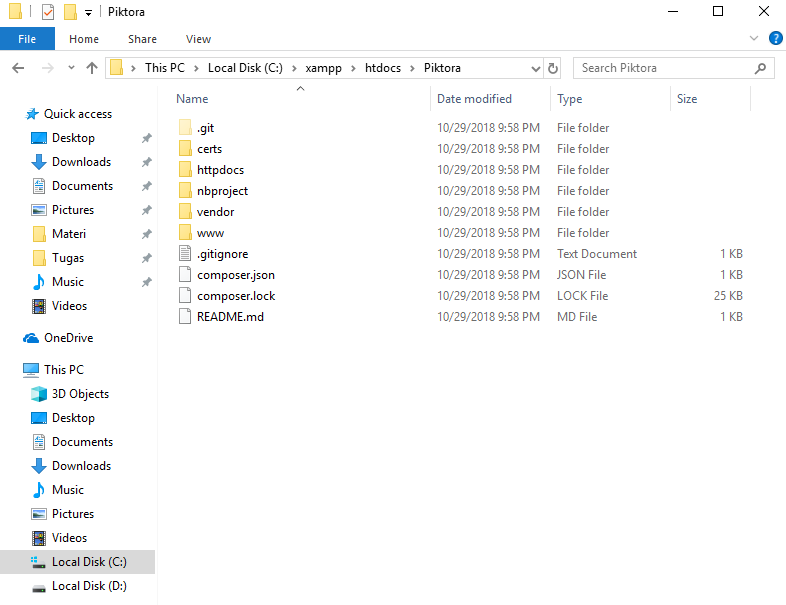
\includegraphics[scale=0.6]{Gambar/piktora_last_commit.png}
	\caption{\textit{Working tree} proyek Piktora pada \textit{commit} terakhir.}
	\label{fig:piktora_last_wt}
\end{figure}
\ \\
Gambar \ref{fig:piktora_last_wt} menunjukkan \textit{working tree} proyek Piktora pada \textit{commit} terakhir. \textit{Folder} git menunjukkan bahwa direktori Piktora terekam oleh Git. \textit{File} dan \textit{folder} yang terdapat pada \textit{working tree} merupakan \textit{snapshot} dari suatu \textit{commit}. Setiap kali dilakukan \textit{checkout}, \textit{working tree} akan berubah sesuai dengan \textit{snapshot} pada \textit{commit} tertentu. Dengan menggunakan operasi \textit{checkout}, dapat dibandingkan \textit{file} versi sekarang dengan \textit{file} pada versi sebelumnya.    
\begin{figure}[H]
	\centering
		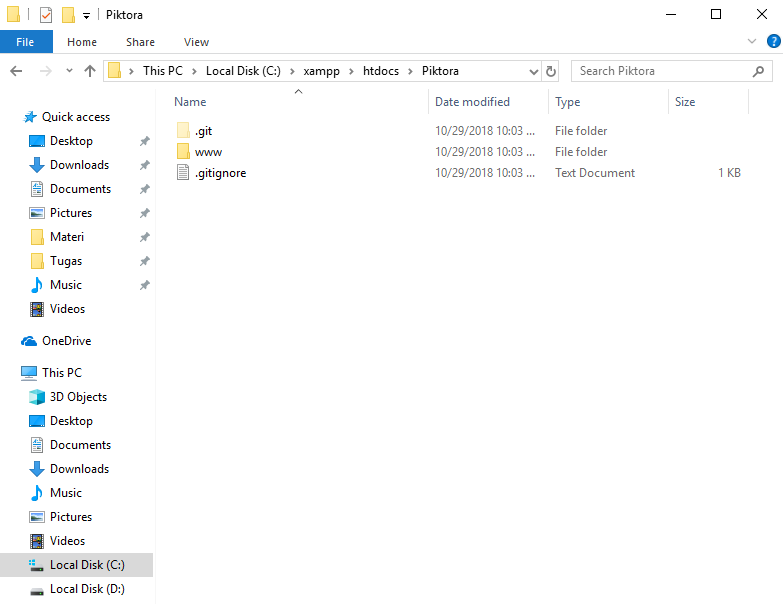
\includegraphics[scale=0.6]{Gambar/piktora_first_commit.png}
	\caption{\textit{Working tree} proyek Piktora pada \textit{commit} pertama.}
	\label{fig:piktora_first_wt}
\end{figure}
\ \\
Gambar \ref{fig:piktora_first_wt} menunjukkan \textit{working tree} proyek Piktora setelah dilakukan \textit{checkout} ke  \textit{commit} pertama. Jika dilihat, terdapat perbedaan \textit{working tree} antara \textit{commit} pertama dan terakhir. Pada \textit{commit} pertama, \textit{working tree} hanya berisi \textit{folder} git, \textit{folder} www, dan \textit{file} file gitignore.  Pada \textit{commit} terakhir, terdapat beberapa \textit{file} dan \textit{folder} baru di \textit{working tree}. 
 
\begin{figure}[H]
	\centering
		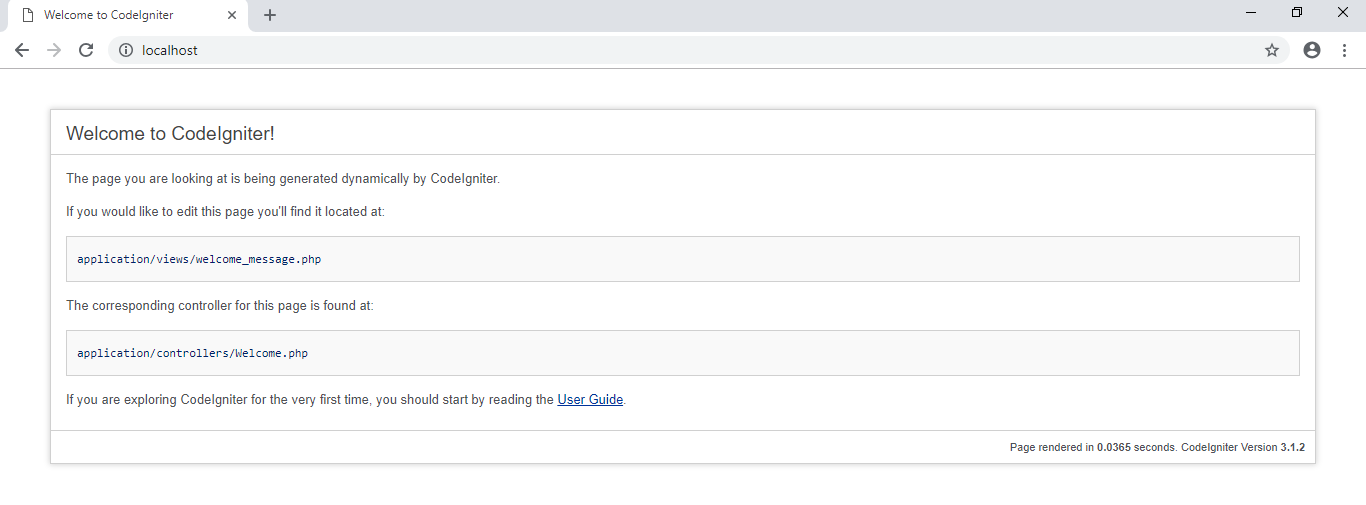
\includegraphics[scale=0.5]{Gambar/piktora_versi_pertama.png}
	\caption{Halaman \textit{web} proyek Piktora pada \textit{commit} pertama.}
	\label{fig:piktora_web_first}
\end{figure} 
\ \\
Selain terdapat perbedaan di \textit{working tree}, terdapat juga perbedaan pada halaman \textit{web} versi pertama dan terakhir. Gambar \ref{fig:piktora_first_wt} menunjukkan halaman \textit{web} Piktora pada \textit{commit} pertama. Gambar \ref{fig:piktora_last_wt} menunjukkan halaman \textit{web} Piktora pada \textit{commit} terakhir.
\begin{figure}[H]
	\centering
		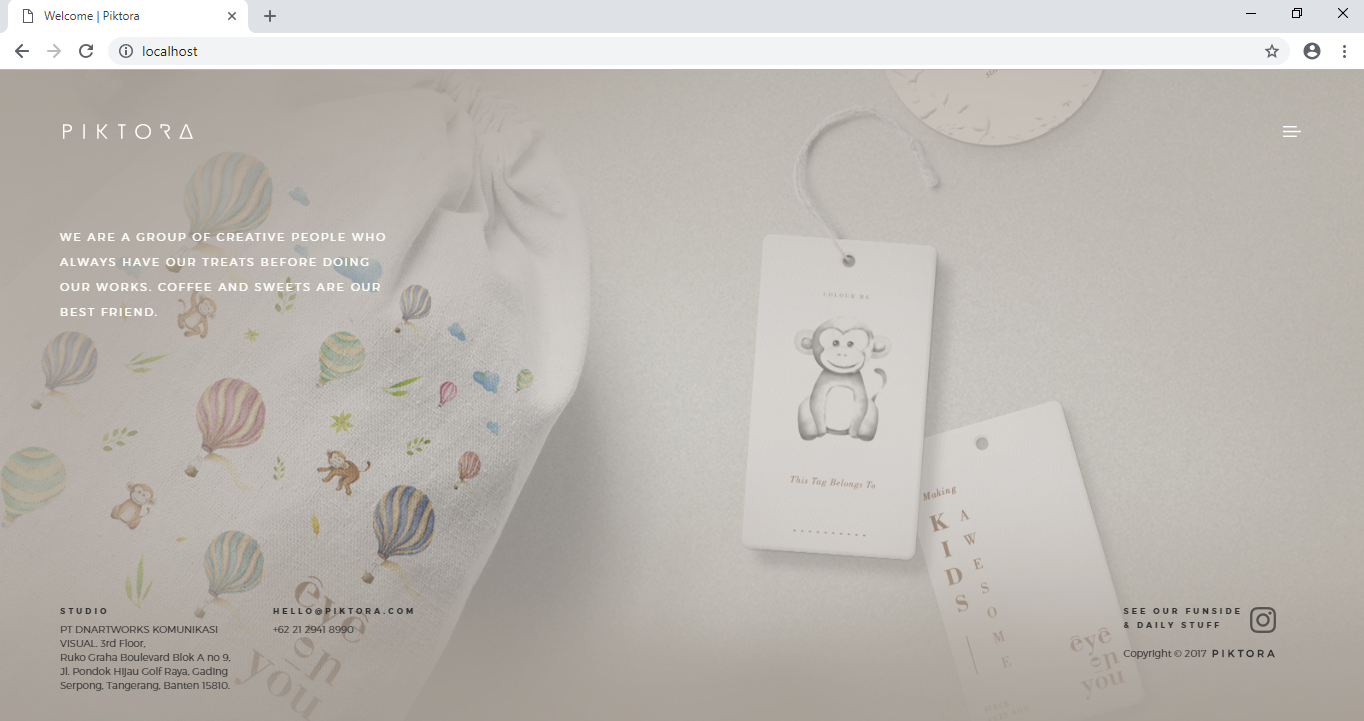
\includegraphics[scale=0.5]{Gambar/piktora_versi_terakhir.png}
	\caption{Halaman \textit{web} proyek Piktora pada \textit{commit} terakhir.}
	\label{fig:piktora_web_last}
\end{figure} 


%\section{Analisis Penggunaan JGit}
%\label{sec:analisis_jgit}

%\section{Analisis Penggunaan Selenium WebDriver}
%\label{sec:analisis_selenium}

%\section{Analisis Penggunaan Apache Commons CLI}
%\label{sec:analisis_apache_commons}

\section{Prapengujian Website Piktora}
\label{sec:prapengujian}
Pengujian dilakukan dengan proyek Piktora sebagai input dari program. Input dari program ini adalah alamat direktori proyek Piktora dan URL untuk membuka halaman \textit{web}. Berikut ini adalah langkah-langkah pada pengujian:\\
\begin{enumerate}
\item Program mengambil input dari parameter menggunakan Apache Commons CLI.
\item Program mendapatkan seluruh \textit{commit} histori dari proyek Piktora menggunakan JGit.
\item Program melakukan \textit{checkout} ke \textit{commit} pertama.
\item Program menjalankan halaman proyek Piktora di \textit{localhost} menggunakan SeleniumWebDriver.
\item SeleniumWebDriver kemudian mengambil \textit{screenshot} pada halaman \textit{web} Piktora.
\item Langkah 3-5 diulangi untuk seluruh \textit{commit}.
\item Menggabungkan semua \textit{file} gambar menjadi satu \textit{file} bertipe GIF.
\end{enumerate}
\ \\

Pada proyek Piktora terdapat 58 \textit{commit}. Listing \ref{lst:all_commit_piktora} menunjukkan histori \textit{commit} pada proyek Piktora. Setelah dilakukan pengujian terdapat beberapa masalah. Masalah tersebut yaitu perbedaan letak \textit{file}, migrasi \textit{database}, dan konfigurasi \textit{database}. Masalah-masalah tersebut dibahas pada subbab \ref{subsec:perbedaan_letak_file} sampai \ref{subsec:migrasi_database}.

\begin{lstlisting}[caption={Histori \textit{commit} pada proyek Piktora},label={lst:all_commit_piktora},language=plaintext]
315d374 -  Oct 31 16:52:46 2016 :  Basic CI files + htaccess & webconfig + database.php ignore

27ce3d4 -  Nov 5 13:12:43 2016 :  setup environment for piktora
65f0c9c -  Nov 5 19:22:58 2016 :  * create structure for all pages * add dummy images

bffbae1 -  Nov 8 18:00:32 2016 :  - basic structure (navbar semi complete) - add fonts

5c59916 -  Nov 8 19:51:18 2016 :  implement navbar, footer, and projects/ page
7738380 -  Nov 8 20:05:27 2016 :  fix pc and ipad navbar fontsize
26bdbee -  Nov 8 20:16:33 2016 :  fix position image for desktop /projects
3db3ce8 -  Nov 9 00:28:27 2016 :  - implements project details page - fix some minor issue - add some project image

5ef34fa -  Nov 13 13:01:06 2016 :  implement about us (raw version)
3caf535 -  Nov 15 11:55:15 2016 :  fix minor issues view/about: - background-image position. Make it to the center position - slick.js img need to set to inline

c5eb3b6 -  Nov 15 13:02:42 2016 :  implement /welcome page
ade9216 -  Nov 15 13:12:08 2016 :  fix minor issues: - move style footer to global - add space before PIKTORA

c77b5b3 -  Nov 18 18:18:25 2016 :  implement /contact
b42b819 -  Nov 18 21:22:22 2016 :  cange a href to style cursor: pointer
3eb7af8 -  Nov 21 16:09:40 2016 :  .htaccess to be compatible with cloud kilat
e87e84b -  Nov 22 14:53:45 2016 :  - change vw to 100% - add captcha
ff8d829 -  Nov 22 15:22:53 2016 :  Solved captcha font load: use otf instead of ttf Also: create directory assets/img/captcha and ignore everything inside

dc87342 -  Nov 22 15:49:03 2016 :  - implement captcha code - remove wrong css
9ebe433 -  Nov 22 16:12:44 2016 :  add scroll feature in project/
f0f7270 -  Nov 23 15:17:42 2016 :  Added Google PHP Client v2 See https://github.com/google/google-api-php-client

57a239b -  Nov 23 15:19:57 2016 :  Merge origin/master
e2dfebe -  Nov 27 14:42:24 2016 :  - remove blue outline when click with slick - change background image in about to newest one

a19e7f2 -  Nov 27 15:24:42 2016 :  Detailing dari Edina: 1. Hal. Project Detail, font coba diperkecil saja mungkin ya. 3. Beberapa ukuran font dan spacing ada yang kurang pas sedikit, terlampir detail revisinya ya (file pdf) 4. Footer dibuat selalu stay terus di bagian bawah dengan posisi yang selalu sama. Di home & contact sudah sama, namun di hal. product posisinya agak lebih naik.

3d79d0a - Nov 27 15:29:58 2016 : fix minor issue
0fcd958 - Nov 28 10:11:06 2016 : add raw admin contents
add3974 - Nov 28 12:03:21 2016 : add summernote, implement read project
0680488 - Nov 29 12:38:23 2016 : update admin for projects
fbe7639 - Nov 29 13:10:30 2016 : implement admin for home
db0cedd - Nov 29 13:38:29 2016 : - implementasi database bagian user - upload 9 gambar contoh project

0fe9aaf - Nov 29 14:17:20 2016 : ubah warna garis captcha
f2326dd - Nov 29 14:44:51 2016 : - lewati proses otentikasi sementara
f78cdb4 - Dec 2 12:10:47 2016 : (trying to) fix issue #2
ef9b62b - Dec 2 17:09:58 2016 : revisi dari edina ke-2
c689aa8 - Dec 2 17:11:13 2016 : perbaikan admin sedikit
c4e9576 - Dec 2 17:14:06 2016 : perbaikan di /contact, kelewat
02d04f1 - Dec 5 14:55:20 2016 : tambah wording
a4e4858 - Dec 5 15:08:59 2016 : perbaikan kata2 sedikit
bbd82c2 - Dec 6 10:41:40 2016 : implementasi email
f8c64fc - Dec 6 11:03:08 2016 : change to httpdocs
eb49c2b - Dec 6 11:35:20 2016 : hapus migrasi script di admin
ace1988 - Dec 6 11:39:00 2016 : change overflow to auto
627e65b - Dec 6 11:45:26 2016 : modify database back to local
0896f81 - Dec 7 16:08:30 2016 : update home versi mobile jadi baru (revisi dari Edina)

5cf1292 - Dec 7 16:21:01 2016 : ubah background di about menjadi tidak pecah
c83f4aa - Thu Dec 15 15:04:30 2016 : remove piktora secrets
57f5ea4 - Thu Dec 15 15:09:43 2016 : remove unimportant data
7931c21 - Dec 24 18:40:41 2016 : edit wording
9b0a302 - Dec 25 06:03:50 2016 : Another wording fix
f1ea410 - Thu Jan 5 15:23:32 2017 : fix instagram link
1880a88 - Thu Jan 5 15:24:12 2017 : Merge branch 'master' of https://github.com/pascalalfadian/Piktora

286aa78 - Jan 16 12:48:45 2017 : Perbaikan wording di admin edit project
33702c2 - Feb 21 13:31:08 2017 : change email sender to piktora@mailgun.dnartworks.com.au

18c39ef - Thu Apr 13 15:21:49 2017 : Test commit (in gitlab). Nothing much important
9bfde3c - Apr 17 15:09:54 2017 : add ignore sftp-config.json
38711f0 - Apr 17 15:15:03 2017 : fix bug ugly display when projects too high
9f041ef - May 15 10:40:16 2017 : set insta url to https://www.instagram.com/piktorastudio/

6a085c1 - Dec 12 14:38:38 2017 : Update company address
89000be - Jan 12 12:25:30 2018 : Update new company address
\end{lstlisting}


\subsection{Perbedaan Letak \textit{File}}
\label{subsec:perbedaan_letak_file}
Pada \textit{commit} 315d374(31 Oktober 2016) s.d. bbd82c2(6 Desember 2016) halaman \textit{web} proyek Piktora tidak bisa dibuka. Hal ini disebabkan oleh perbedaan letak \textit{file} "index.php". Pada \textit{commit} 315d374(31 Oktober 2016) s.d. bbd82c2(6 Desember 2016), \textit{file} "index.php" berada pada \textit{folder} "www", sedangkan pada \textit{commit} f8c64fc(6 Desember 2016) s.d. 89000be(12 Januari 2018) \textit{file} "index.php" berada pada \textit{folder} "httpdocs".

Solusi untuk mengatasi masalah ini adalah dengan menambahkan \textit{command line options} yang menerima sebuah \textit{script} PHP. \textit{Script} PHP ini akan mengecek letak \textit{file} "index.php" pada \textit{folder} "www" dan "httpdocs". \textit{Script} kemudian akan mengecek \textit{directory root} XAMPP pada \textit{file} "httpd.conf".  Jika \textit{directory root} sudah mengarah ke \textit{folder} tempat "index.php" berada, maka \textit{script} tidak akan mengubah isi \textit{file} "httpd.conf". Jika \textit{directory root} tidak mengarah ke \textit{folder} tempat "index.php" berada, maka \textit{script} akan mengubah \textit{directory root} pada \textit{file} "httpd.conf". Setelah itu, \textit{script} akan menjalankan perintah "httpd -k restart" untuk melakukan \textit{restart} pada XAMPP. \textit{Script} PHP ini akan dijalankan sebelum melakukan migrasi \textit{database}.   


\subsection{Permasalahan Konfigurasi \textit{Database}}
\label{subsec:konfigurasi_database}
Pada \textit{commit} f8c64fc(6 Desember 2016) s.d. ace1988(6 Desember 2016), halaman \textit{web} tidak bisa dibuka. Hal ini disebabkan karena perbedaan konfigurasi pada \textit{file} "database.php". Pada \textit{commit} f8c64fc(6 Desember 2016) s.d. 57f5ea4(15 Desember 2016) dan \textit{commit} f1ea410(5 Januari 2017), di dalam \textit{file} "database.php" terdapat \textit{password} . \textit{Commit} lainnya tidak terdapat \textit{password} pada \textit{file} "database.php". Penulis menggunakan \textit{password} \texttt{"piktora"} pada konfigurasi \textit{database} di XAMPP.

\begin{lstlisting}[caption={Isi \textit{file} "database.php" pada \textit{commit} f8c64fc(6 Desember 2016)},label={lst:piktora_commit_f8c64fc},language=plaintext]
$active_group = 'default';
$query_builder = TRUE;

$db['default'] = array(
	'dsn'	=> '',
	'hostname' => 'localhost',
	'username' => 'piktora',
	'password' => 'dmHx64%6',
	'database' => 'piktora',
	'dbdriver' => 'mysqli',
	'dbprefix' => '',
	'pconnect' => FALSE,
	'db_debug' => (ENVIRONMENT !== 'production'),
	'cache_on' => FALSE,
	'cachedir' => '',
	'char_set' => 'utf8',
	'dbcollat' => 'utf8_general_ci',
	'swap_pre' => '',
	'encrypt' => FALSE,
	'compress' => FALSE,
	'stricton' => FALSE,
	'failover' => array(),
	'save_queries' => TRUE
);
\end{lstlisting}

Listing \ref{lst:piktora_commit_f8c64fc} merupakan isi dari \textit{file} "database.php" pada \textit{commit} f8c64fc(6 Desember 2016). Dapat dilihat bahwa \textit{password} yang terdapat pada \textit{file} "database.php" adalah \texttt{dmHx64\%6}. \textit{Commit} f8c64fc(6 Desember 2016) s.d. ace1988(6 Desember 2016) menggunakan \textit{password} \texttt{dmHx64\%6}, sedangkan \textit{commit} 627e65b(6 Desember 2016) s.d. 57f5ea4(15 Desember 2016) dan f1ea410(5 Januari 2017) menggunakan \textit{password} \texttt{piktora}. Karena konfigurasi \textit{password} pada \textit{file} "database.php" dan XAMPP berbeda, halaman \textit{website} pada \textit{commit} f8c64fc(6 Desember 2016) s.d. ace1988(6 Desember 2016) tidak bisa dibuka. 

Sama seperti subbab \ref{subsec:perbedaan_letak_file}, solusi untuk mengatasi masalah ini adalah dengan menambahkan \textit{command line options} yang menerima sebuah \textit{script} PHP. \textit{Script} ini akan mengecek \textit{password} yang terdapat pada \textit{file} "database.php". Jika tidak ditemukan \textit{password} atau ditemukan \textit{password} berupa \texttt{piktora}, maka \textit{script} tidak akan mengubah isi \textit{file} "database.php". Jika ditemukan \textit{password} berupa \texttt{dmHx64\%6}, maka \textit{script} akan mengubah \textit{password} menjadi \texttt{piktora}. 

 \subsection{Permasalahan Migrasi \textit{Database}}
\label{subsec:migrasi_database}

Pada \textit{commit} 3d79d0a(27 Nov 2016), terjadi \textit{error} saat melakukan migrasi database. Pada \textit{commit} a19e7f2(27 November 2016), terdapat satu \textit{file} untuk melakukan migrasi yaitu "20161122150000\_Structure.php". Pada \textit{commit} 3d79d0a(27 Nov 2016) terdapat dua \textit{file} untuk melakukan migrasi yaitu "20161122150000\_Structure.php" dan "20161122150001\_InitialData.php". Pada \textit{commit} a19e7f2(27 November 2016) \textit{file} "20161122150001\_InitialData.php" dijalankan saat melakukan migrasi. Versi migrasi \textit{database} menjadi "20161122150000". Pada \textit{commit} 3d79d0a(27 Nov 2016), \textit{file} "20161122150000\_Structure.php" tidak dijalankan karena dianggap sama dengan versi migrasi \textit{database} saat ini. Hanya \textit{file} "20161122150001\_InitialData.php" yang dijalankan pada \textit{commit} 3d79d0a(27 Nov 2016). Isi \textit{file} "20161122150001\_InitialData.php" pada \textit{commit} a19e7f2(27 November 2016) dan 3d79d0a(27 Nov 2016) berbeda. Hal ini yang menyebabkan terjadinya \textit{error} saat melakukan migrasi database.  

Sama seperti subbab \ref{subsec:perbedaan_letak_file}, solusi untuk mengatasi masalah ini adalah dengan menambahkan \textit{command line options} yang menerima sebuah \textit{script} PHP. \textit{Script} ini akan melakukan dua pekerjaan. Pertama, \textit{script} akan menghapus \textit{database} piktora dengan menggunakan \textit{query} "DROP DATABASE piktora". Setelah itu \textit{script} akan membuat \textit{database} piktora dengan menggunakan \textit{query} "CREATE DATABASE piktora". \textit{Script} akan dijalankan sebelum melakukan migrasi \textit{database}. 

\section{Analisis Command Line Options}
\label{sec:analisis_command_line_options}
Program pada skripsi ini akan menerima masukan dari Command Line Options. Selain itu konfigurasi program juga didapatkan dari Command Line Options. Berikut ini adalah \textit{command line options} yang akan diimplementasikan pada skripsi ini:
\begin{enumerate}
\item \texttt{-project-path [PATH]}\\
Opsi ini berfungsi untuk mengatur \textit{path} dari direktori yang akan dibuat animasinya. Parameter dari opsi ini adalah \textit{path} dari proyek perangkat lunak web yang terekam oleh Git. Opsi ini wajib ada.

\item \texttt{-before-capture [PHP-SCRIPT]}\\
Opsi ini berfungsi untuk menjalankan \textit{script} PHP. \textit{Script} ini dijalankan sebelum melakukan \textit{screenshot}. Parameter dari opsi ini adalah \textit{script} PHP. Opsi ini bersifat opsional.

\item \texttt{-capture-url [url]}\\
Opsi ini berfungsi untuk mengatur alamat \textit{url} dari halaman \textit{web}, dimana dilakukan pengambilan \textit{screenshot} pada halaman ini. Parameter dari opsi ini adalah alamat \textit{url} dari halaman \textit{web}. Opsi ini wajib ada.

\item \texttt{-fps [FPS]}\\
Opsi ini berfungsi untuk mengatur jumlah \textit{frame} per detik pada animasi.  Parameter dari opsi ini adalah jumlah \textit{frame} per detik. Opsi ini bersifat opsional.

\item \texttt{-title [TITLE]}\\
Opsi ini berfungsi untuk memberi judul. Opsi ini bersifat opsional. 

\item \texttt{-logo [IMAGE]}\\
Opsi ini berfungsi untuk memasukkan logo. Parameter dari opsi ini adalah \textit{file} gambar. Opsi ini bersifat opsional.

\item \texttt{-start-commit [ID] -stop-commit [ID]}\\
Opsi ini berfungsi untuk mengatur rentang \textit{commit} yang akan dibuat animasinya. Parameter dari opsi ini adalah \textit{commit ID} awal dan \textit{commit ID} akhir. Opsi ini bersifat opsional. 
\end{enumerate}
